\documentclass{article}

\usepackage{tikz}
\usepackage{pgfplots}
\begin{document}

\section{Scalability}

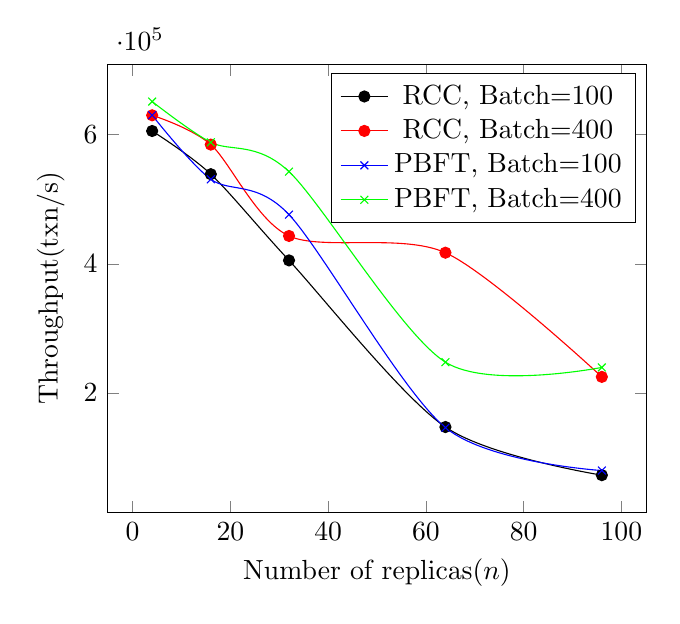
\begin{tikzpicture}
    \begin{axis}[
        xlabel= Number of replicas$(n)$,
        ylabel= Throughput(txn/s)]
    \addplot[smooth,mark=*,black] 
        plot coordinates {
            (4,605740)
            (16,538840)
            (32,405280)
            (64,147120)
            (96,72540)
    };
    \addlegendentry{RCC, Batch=100}

    \addplot[smooth,mark=*,red] 
        plot coordinates {
            (4,630080)
            (16,584640)
            (32,443120)
            (64,417200)
            (96, 224800)
    };
    \addlegendentry{RCC, Batch=400}

    \addplot[smooth,color=blue,mark=x]
        plot coordinates {
            (4,630220)
            (16,531000)
            (32,476160)
            (64,146220)
            (96,79700)
        };
    \addlegendentry{PBFT, Batch=100}

    \addplot[smooth,color=green,mark=x]
        plot coordinates {
            (4,651360)
            (16,588160)
            (32,542800)
            (64,247600)
            (96,239440)
        };
    \addlegendentry{PBFT, Batch=400}
  
    \end{axis}
    \end{tikzpicture}


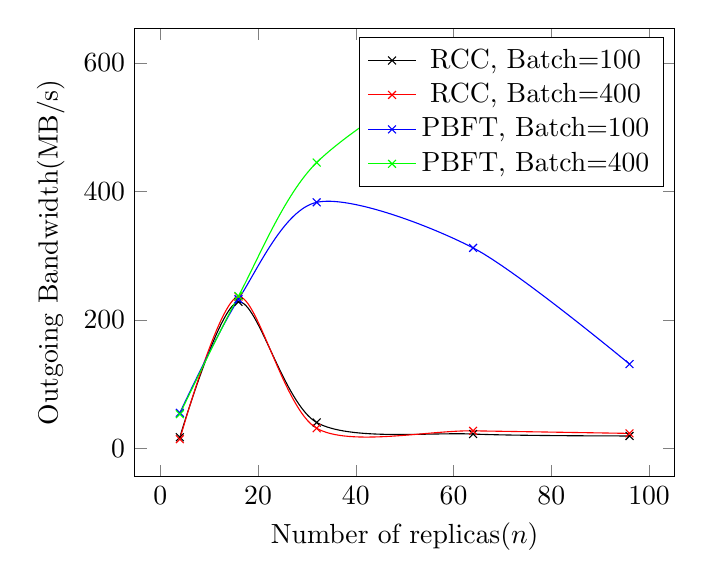
\begin{tikzpicture}
    \begin{axis}[
        xlabel= Number of replicas$(n)$,
        ylabel= Outgoing Bandwidth(MB/s)]

    \addplot[smooth,color=black,mark=x]
        plot coordinates {
            (4,17)
            (16,228)
            (32,40)
            (64,22)
            (96,19)
        };
    \addlegendentry{RCC, Batch=100}

        \addplot[smooth,color=red,mark=x]
        plot coordinates {
            (4,14)
            (16,236)
            (32,31)
            (64,27)
            (96,23)
        };
    \addlegendentry{RCC, Batch=400} 

    \addplot[smooth,color=blue,mark=x]
        plot coordinates {
            (4,55)
            (16,232)
            (32,383)
            (64,312)
            (96,131)
        };
    \addlegendentry{PBFT, Batch=100} 

    \addplot[smooth,color=green,mark=x]
        plot coordinates {
            (4,53)
            (16,237)
            (32,445)
            (64,596)
            (96,593)
        };
    \addlegendentry{PBFT, Batch=400}
    \end{axis}
    \end{tikzpicture}




\section{BatchSize}
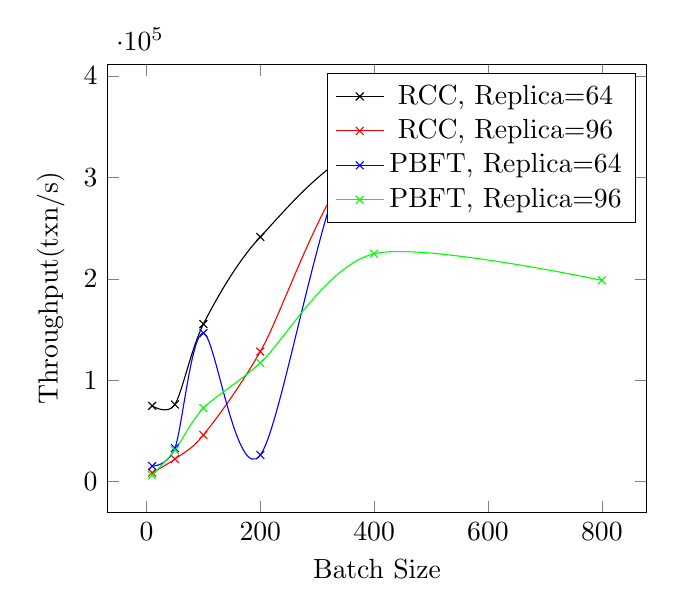
\begin{tikzpicture}
    \begin{axis}[
        xlabel= Batch Size,
        ylabel= Throughput(txn/s)]

    \addplot[smooth,color=black,mark=x]
        plot coordinates {
            (10,74800)
            (50,76160)
            (100,155420)
            (200,241320)
            (400,334640)
            (800,358400)       
        };
    \addlegendentry{RCC, Replica=64}

    \addplot[smooth,color=red,mark=x]
        plot coordinates {
            (10,8834)
            (50,22420)
            (100,46080)
            (200,128320)
            (400,336320)
            (800,374800)       
        };
    \addlegendentry{RCC, Replica=96}

    \addplot[smooth,color=blue,mark=x]
        plot coordinates {
            (10,15400)
            (50,33250)
            (100,146520)
            (200,26330)
            (400,372960)
            (800,358720)       
        };
    \addlegendentry{PBFT, Replica=64}

    \addplot[smooth,color= green,mark=x]
        plot coordinates {
            (10,6466)
            (50,31260)
            (100,72540)
            (200,117200)
            (400,224800)
            (800,198560)       
        };
    \addlegendentry{PBFT, Replica=96}
    \end{axis}
    \end{tikzpicture}

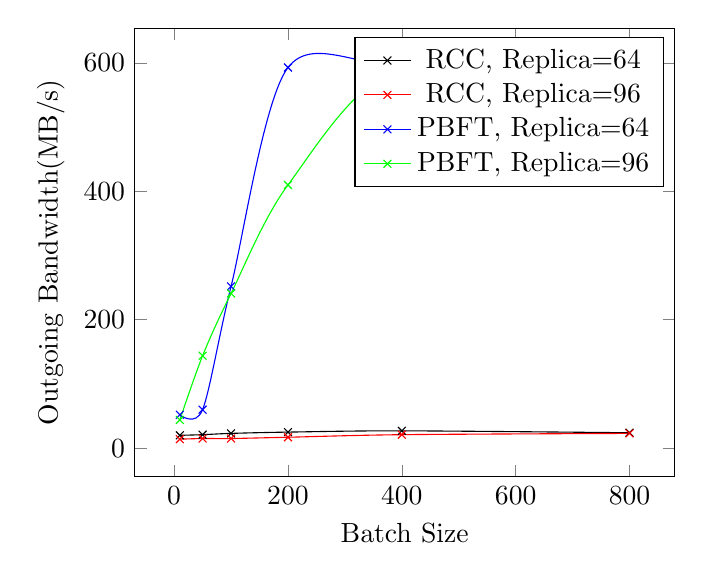
\begin{tikzpicture}
    \begin{axis}[
        xlabel= Batch Size,
        ylabel= Outgoing Bandwidth(MB/s)]

    \addplot[smooth,color=black,mark=x]
        plot coordinates {
            (10,20)
            (50,21)
            (100,23)
            (200,25)
            (400,27)
            (800,24)       
        };
    \addlegendentry{RCC, Replica=64}

    \addplot[smooth,color=red,mark=x]
        plot coordinates {
            (10,14)
            (50,15)
            (100,15)
            (200,17)
            (400,21)
            (800,23)       
        };
    \addlegendentry{RCC, Replica=96}

    \addplot[smooth,color=blue,mark=x]
        plot coordinates {
            (10,52)
            (50,60)
            (100,252)
            (200,593)
            (400,596)
            (800,596)       
        };
    \addlegendentry{PBFT, Replica=64}

    \addplot[smooth,color= green,mark=x]
        plot coordinates {
            (10,44)
            (50,144)
            (100,241)
            (200,410)
            (400,596)
            (800,596)       
        };
    \addlegendentry{PBFT, Replica=96}
    \end{axis}
    \end{tikzpicture}

\section{Concurrency}
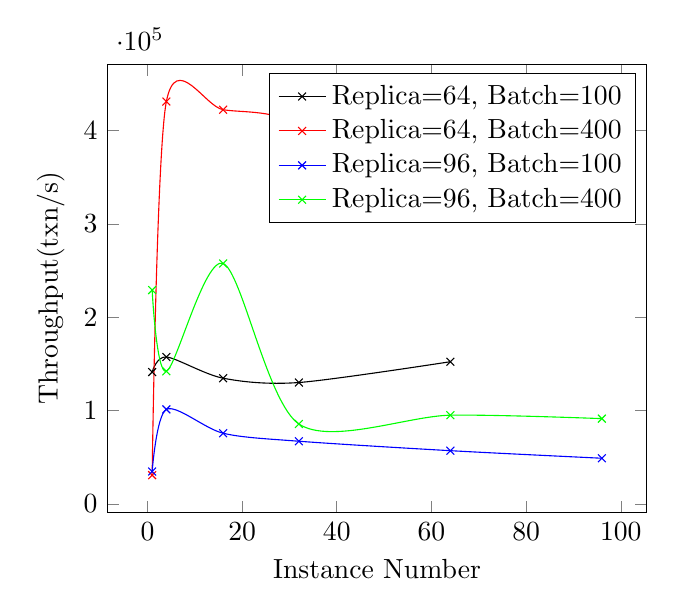
\begin{tikzpicture}
    \begin{axis}[
        xlabel= Instance Number,
        ylabel= Throughput(txn/s)]

    \addplot[smooth,color=black,mark=x]
        plot coordinates {
            (1,141180)
            (4,157360)
            (16,134600)
            (32,129980)
            (64,152280)       
        };
    \addlegendentry{Replica=64, Batch=100}

    \addplot[smooth,color=red,mark=x]
        plot coordinates {
            (1,30680)
            (4,431120)
            (16,422400)
            (32,407740)
            (64,317280)       
        };
    \addlegendentry{Replica=64, Batch=400}

    \addplot[smooth,color=blue,mark=x]
        plot coordinates {
            (1,34560)
            (4,101180)
            (16,75620)
            (32,67040)
            (64,56920)
            (96,48820)
        };
    \addlegendentry{Replica=96, Batch=100}

    \addplot[smooth,color= green,mark=x]
        plot coordinates {
            (1,229040)
            (4,142000)
            (16,257600)
            (32,85520)
            (64,94960)
            (96,91280)
        };
    \addlegendentry{Replica=96, Batch=400}
    \end{axis}
    \end{tikzpicture}

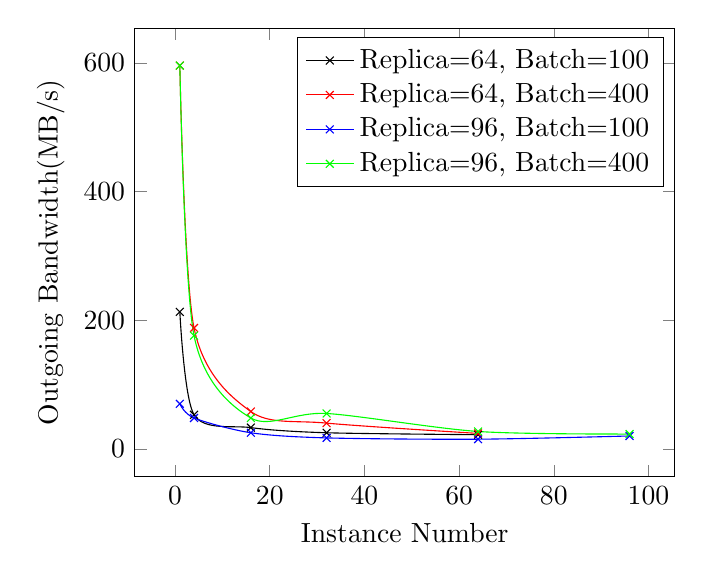
\begin{tikzpicture}
    \begin{axis}[
        xlabel= Instance Number,
        ylabel= Outgoing Bandwidth(MB/s)]

    \addplot[smooth,color=black,mark=x]
        plot coordinates {
            (1,213)
            (4,53)
            (16,33)
            (32,25)
            (64,22)       
        };
    \addlegendentry{Replica=64, Batch=100}

    \addplot[smooth,color=red,mark=x]
        plot coordinates {
            (1,596)
            (4,188)
            (16,58)
            (32,40)
            (64,24)       
        };
    \addlegendentry{Replica=64, Batch=400}

    \addplot[smooth,color=blue,mark=x]
        plot coordinates {
            (1,70)
            (4,48)
            (16,25)
            (32,17)
            (64,15) 
            (96,20)
        };
    \addlegendentry{Replica=96, Batch=100}

    \addplot[smooth,color= green,mark=x]
        plot coordinates {
            (1,596)
            (4,176)
            (16,48)
            (32,55)
            (64,27)
            (96,23)
        };
    \addlegendentry{Replica=96, Batch=400}
    \end{axis}
    \end{tikzpicture}
    
\end{document}
